\documentclass[uplatex,dvipdfmx,a4paper]{jsarticle}

\usepackage[margin=0mm]{geometry}
\usepackage[dvipdfmx]{graphicx,xcolor,hyperref}
\usepackage{pxjahyper}
\usepackage{tikz}
\usepackage{qrcode}
\usetikzlibrary{calc,positioning}

\pagestyle{empty}
\setlength{\parindent}{0pt}

\definecolor{Navy}{HTML}{071325}
\definecolor{NavySoft}{HTML}{17304F}
\definecolor{Cream}{HTML}{F4F1E8}
\definecolor{White}{HTML}{FFFDF7}
\definecolor{Amber}{HTML}{FFC86A}
\definecolor{Gold}{HTML}{947027}
\definecolor{InkSoft}{HTML}{485361}
\definecolor{Rule}{HTML}{D2CABB}

\hypersetup{
  colorlinks=true,
  urlcolor=NavySoft,
  pdftitle={橋田ゼミ冬の音楽展2026 チラシ初稿},
  pdfauthor={福知山公立大学 橋田ゼミ}
}

\newcommand{\sans}{\sffamily}
\newcommand{\serif}{\rmfamily}

\begin{document}
\begin{tikzpicture}[remember picture,overlay]
  % Base
  \fill[Cream] (current page.south west) rectangle (current page.north east);

  % Winter visual
  \begin{scope}
    \clip (current page.north west) rectangle ([yshift=-126mm]current page.north east);
    \node[anchor=north,inner sep=0pt] at (current page.north) {%
      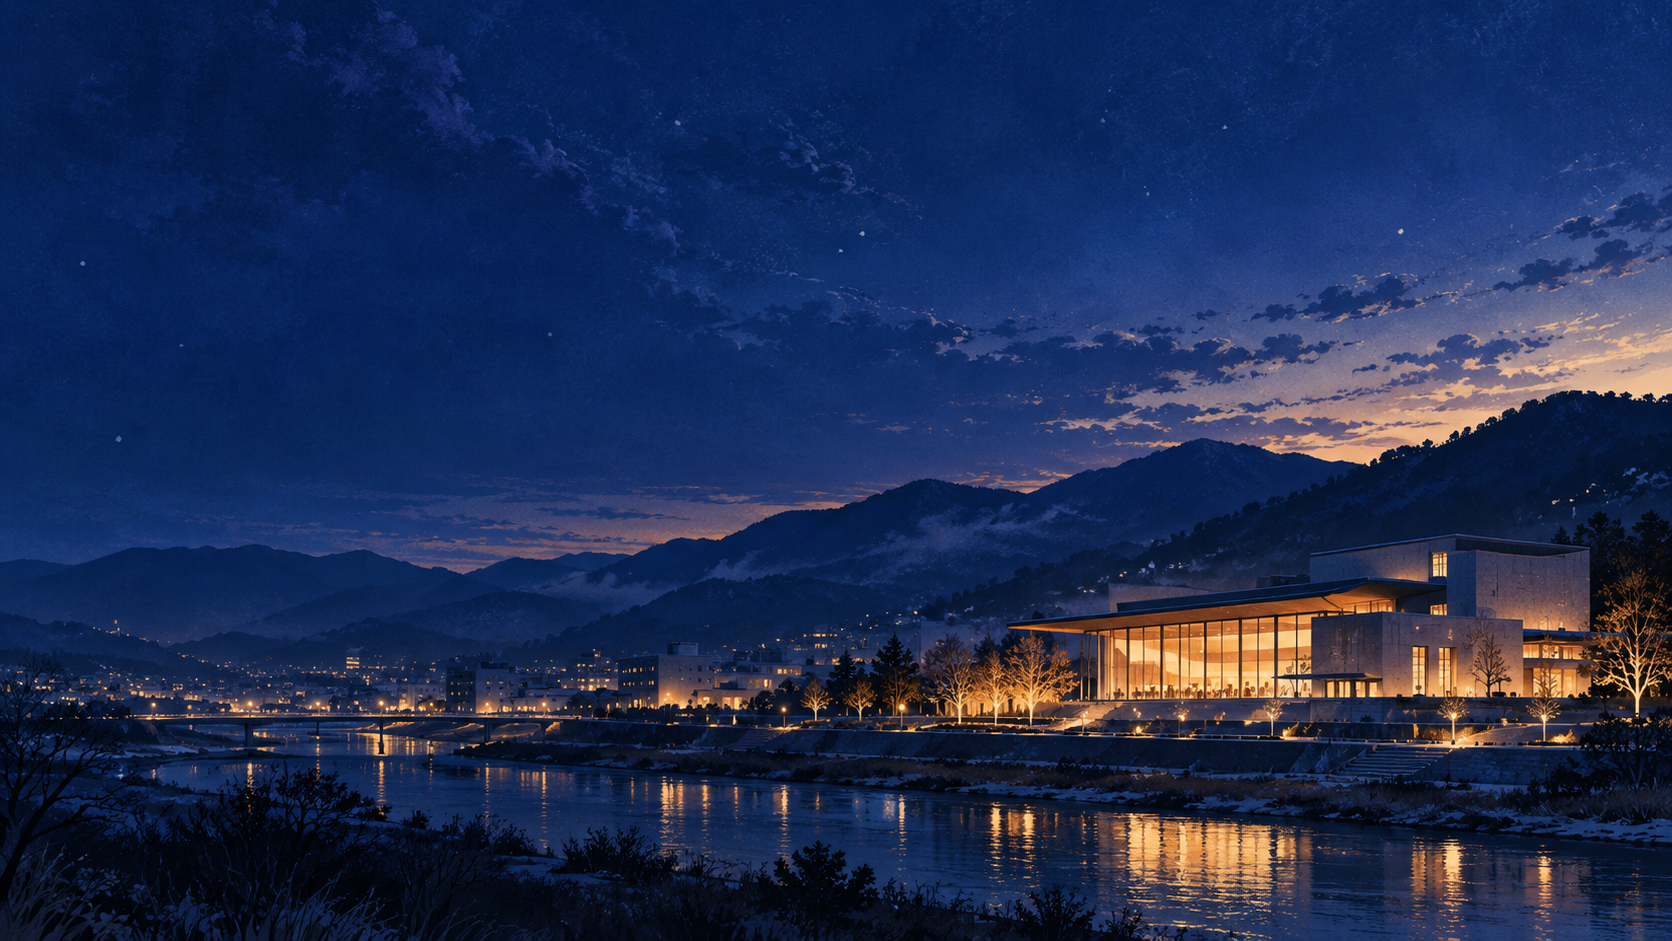
\includegraphics[width=\paperwidth,height=126mm]{../assets/winter-fukuchiyama.png}};
    \shade[left color=Navy,right color=Navy!20,opacity=0.84]
      (current page.north west) rectangle ([yshift=-126mm]current page.north east);
    \fill[Navy,opacity=0.24]
      (current page.north west) rectangle ([yshift=-126mm]current page.north east);
  \end{scope}

  % Top identity
  \node[anchor=north west,text=White,font=\sans\bfseries\fontsize{10}{12}\selectfont]
    at ([xshift=17mm,yshift=-13mm]current page.north west)
    {福知山公立大学　橋田ゼミ};
  \node[anchor=north west,text=Amber,font=\sans\bfseries\fontsize{6.5}{8}\selectfont]
    at ([xshift=17mm,yshift=-21mm]current page.north west)
    {HASHIDA LAB / WINTER MUSIC EXHIBITION};

  \node[anchor=north east,inner sep=0pt]
    at ([xshift=-15mm,yshift=-12mm]current page.north east)
    {
\includegraphics[width=15mm]{../企画書/assets/fpu-logomark.png}};

  % Status label
  \node[anchor=north west,rounded corners=7pt,fill=Amber,text=Navy,
        inner xsep=9pt,inner ysep=4.5pt,font=\sans\bfseries\fontsize{8}{9}\selectfont]
    at ([xshift=17mm,yshift=-34mm]current page.north west)
    {一般公開　｜　開催決定};

  % Main title
  \node[anchor=north west,text=White,text width=168mm,align=left,font=\serif\bfseries\Huge]
    at ([xshift=16mm,yshift=-48mm]current page.north west)
    {橋田ゼミ冬の音楽展2026};

  \node[anchor=north west,text=White!82,text width=150mm,align=left,
        font=\serif\fontsize{13}{18}\selectfont]
    at ([xshift=18mm,yshift=-72mm]current page.north west)
    {研究と音楽。学びを、まちにひらく。};

  % Date block
  \draw[Amber,line width=0.7pt]
    ([xshift=17mm,yshift=-95mm]current page.north west) --
    ([xshift=193mm,yshift=-95mm]current page.north west);
  \node[anchor=north west,text=White,font=\serif\bfseries]
    at ([xshift=17mm,yshift=-97mm]current page.north west)
    {{\fontsize{33}{35}\selectfont 12.15}\hspace{3mm}
     {\sans\fontsize{10}{12}\selectfont TUE}};
  \node[anchor=north east,text=White,align=right,font=\sans\fontsize{10}{14}\selectfont]
    at ([xshift=-17mm,yshift=-101mm]current page.north east)
    {2026年\quad 福知山サンホテル\, 扇ホール};

  % Lower section heading
  \node[anchor=north west,text=Gold,font=\sans\bfseries\fontsize{7}{8}\selectfont]
    at ([xshift=17mm,yshift=-134mm]current page.north west)
    {PROGRAM / 予定プログラム};

  % Program cards
  \fill[White,rounded corners=2pt]
    ([xshift=17mm,yshift=-143mm]current page.north west) rectangle
    ([xshift=101mm,yshift=-176mm]current page.north west);
  \fill[NavySoft,rounded corners=2pt]
    ([xshift=105mm,yshift=-143mm]current page.north west) rectangle
    ([xshift=193mm,yshift=-176mm]current page.north west);

  \node[anchor=north west,text=Gold,font=\sans\bfseries\fontsize{6.5}{8}\selectfont]
    at ([xshift=23mm,yshift=-149mm]current page.north west) {MORNING / 午前};
  \node[anchor=north west,text=Navy,font=\serif\bfseries\fontsize{16}{20}\selectfont]
    at ([xshift=23mm,yshift=-157mm]current page.north west) {研究中間発表};
  \node[anchor=north west,text=InkSoft,font=\sans\fontsize{7}{9}\selectfont]
    at ([xshift=23mm,yshift=-168mm]current page.north west) {3・4年生による研究発表を予定};

  \node[anchor=north west,text=Amber,font=\sans\bfseries\fontsize{6.5}{8}\selectfont]
    at ([xshift=112mm,yshift=-149mm]current page.north west) {AFTERNOON / 午後};
  \node[anchor=north west,text=White,font=\serif\bfseries\fontsize{16}{20}\selectfont]
    at ([xshift=112mm,yshift=-157mm]current page.north west) {合同企画・音楽演奏};
  \node[anchor=north west,text=White!68,font=\sans\fontsize{7}{9}\selectfont]
    at ([xshift=112mm,yshift=-168mm]current page.north west) {学生が一つの演奏をつくり上げます};

  % Song highlight
  \fill[Amber!26,rounded corners=2pt]
    ([xshift=17mm,yshift=-181mm]current page.north west) rectangle
    ([xshift=193mm,yshift=-205mm]current page.north west);
  \node[anchor=west,text=Gold,font=\sans\bfseries\fontsize{6.5}{8}\selectfont]
    at ([xshift=23mm,yshift=-193mm]current page.north west) {PERFORMING};
  \node[anchor=west,text=Navy,font=\serif\bfseries\fontsize{15}{18}\selectfont]
    at ([xshift=52mm,yshift=-193mm]current page.north west)
    {Mrs. GREEN APPLE「点描の唄」};

  % Venue photograph
  \begin{scope}
    \clip ([xshift=17mm,yshift=-212mm]current page.north west) rectangle
          ([xshift=98mm,yshift=-260mm]current page.north west);
    \node[anchor=north,inner sep=0pt]
      at ([xshift=57.5mm,yshift=-212mm]current page.north west)
      {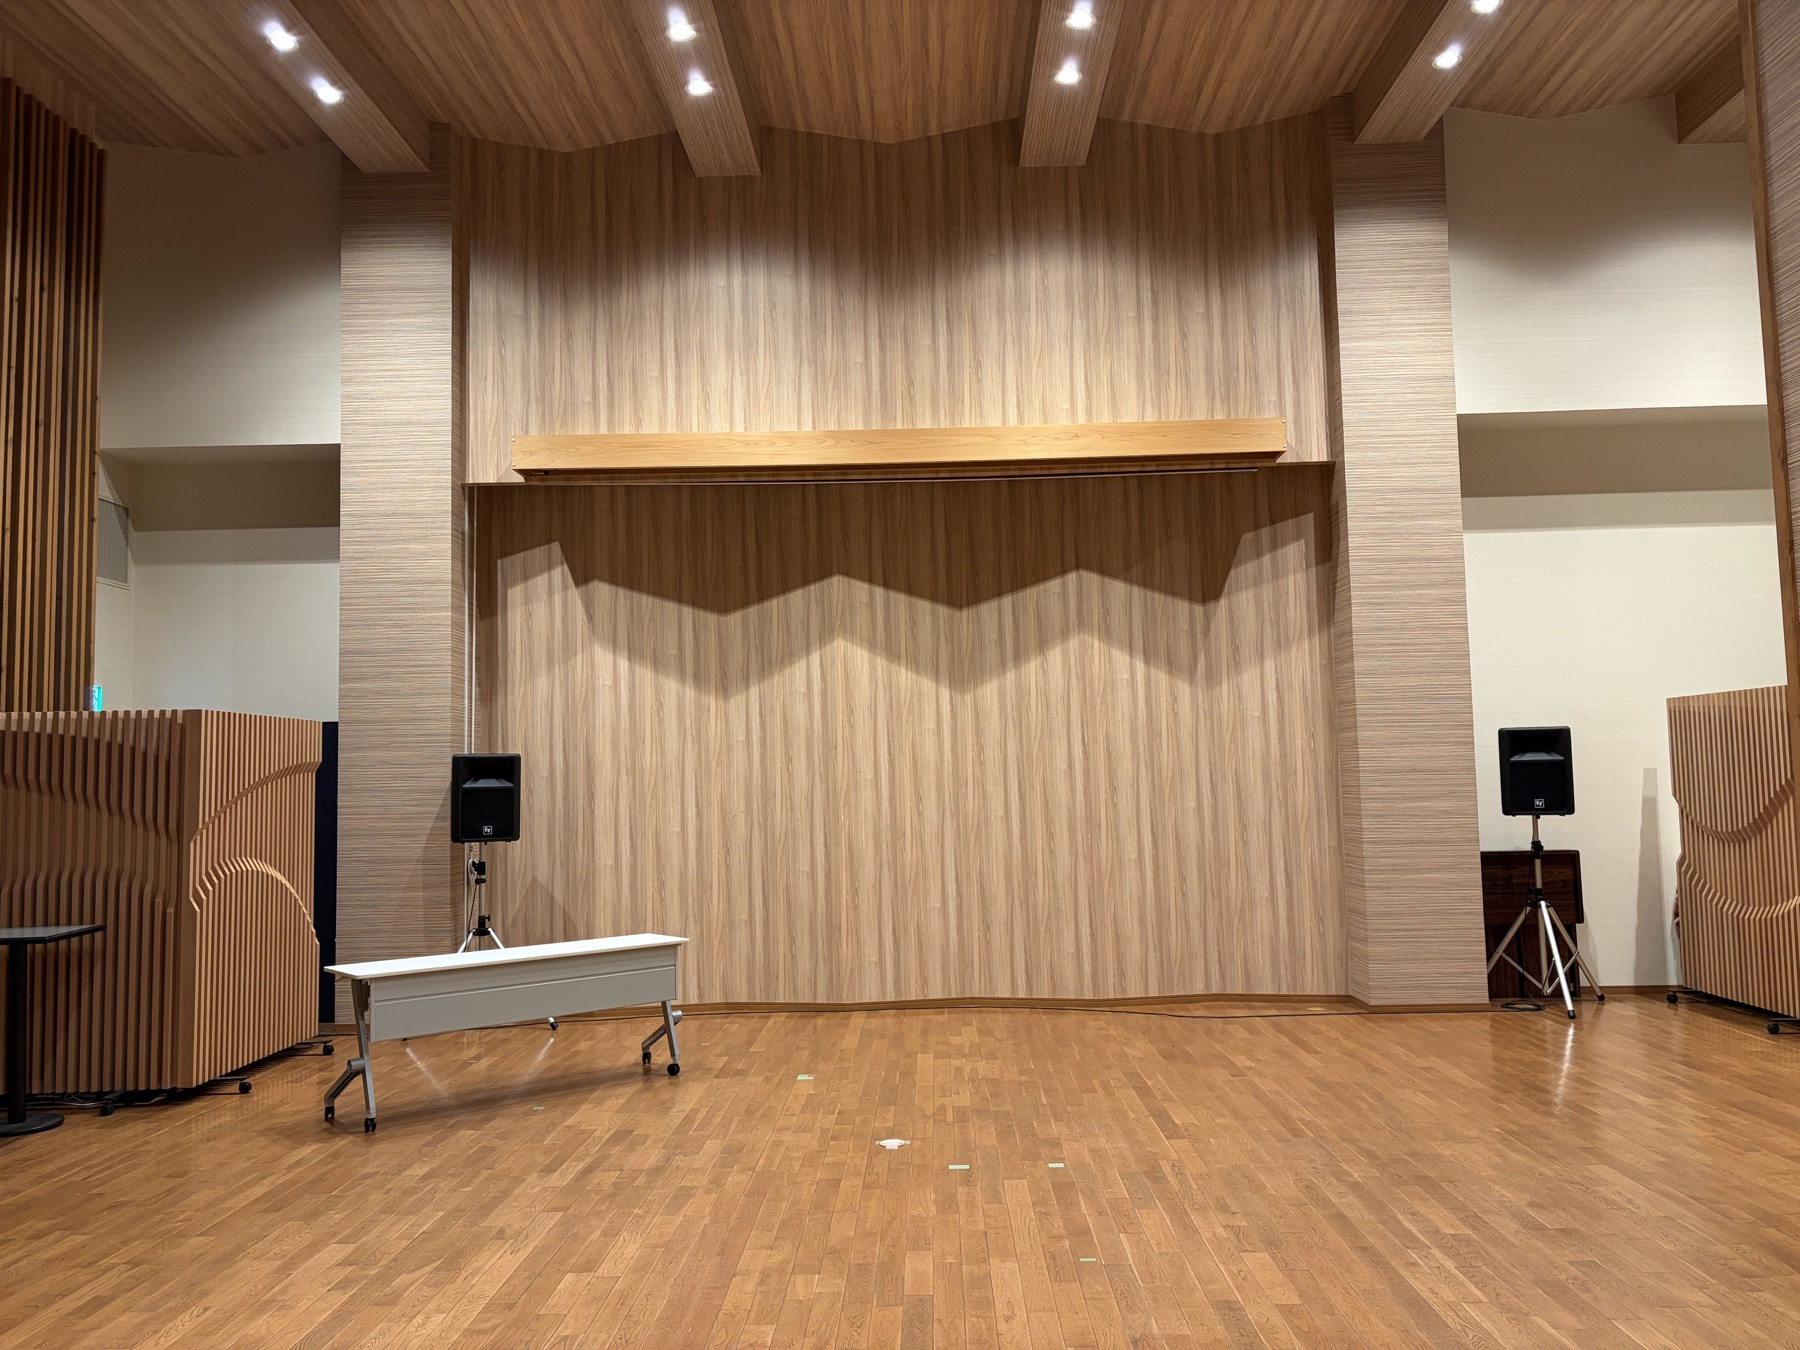
\includegraphics[width=81mm,height=48mm]{../assets/ogihall-stage.jpg}};
  \end{scope}
  \node[anchor=south west,fill=Navy,fill opacity=0.82,text opacity=1,text=White,
        inner xsep=5pt,inner ysep=3pt,font=\sans\bfseries\fontsize{6}{7}\selectfont]
    at ([xshift=17mm,yshift=-260mm]current page.north west)
    {本番会場・扇ホール};

  % Venue text and QR
  \node[anchor=north west,text=Gold,font=\sans\bfseries\fontsize{6.5}{8}\selectfont]
    at ([xshift=105mm,yshift=-213mm]current page.north west) {VENUE / 会場};
  \node[anchor=north west,text=Navy,text width=82mm,align=left,font=\serif\bfseries]
    at ([xshift=105mm,yshift=-221mm]current page.north west)
    {{\fontsize{15}{19}\selectfont 福知山サンホテル\quad 扇ホール}};
  \node[anchor=north west,text=InkSoft,text width=60mm,align=left,
        font=\sans\fontsize{7}{10}\selectfont]
    at ([xshift=105mm,yshift=-237mm]current page.north west)
    {〒620-0882 京都府福知山市堀2080\\
     開場・開演時刻、参加方法、入場料は\\
     決まり次第Webサイトでご案内します。};

  \node[anchor=north east,inner sep=0pt]
    at ([xshift=-17mm,yshift=-229mm]current page.north east)
    {\href{https://ryu-mei-15.github.io/HashidaLabWinterPresentation/}{%
      \qrcode[height=24mm]{https://ryu-mei-15.github.io/HashidaLabWinterPresentation/}}};
  \node[anchor=north,text=Gold,font=\sans\bfseries\fontsize{6}{7}\selectfont]
    at ([xshift=-29mm,yshift=-218mm]current page.north east)
    {最新情報・詳細};

  % Footer
  \draw[Rule,line width=0.4pt]
    ([xshift=17mm,yshift=-267mm]current page.north west) --
    ([xshift=193mm,yshift=-267mm]current page.north west);
  \node[anchor=north west,text=Navy,font=\sans\bfseries\fontsize{8}{10}\selectfont]
    at ([xshift=17mm,yshift=-273mm]current page.north west)
    {福知山公立大学　橋田ゼミ};
  \node[anchor=north west,text=InkSoft,text width=130mm,align=left,
        font=\sans\fontsize{6.3}{9}\selectfont]
    at ([xshift=17mm,yshift=-282mm]current page.north west)
    {内容は2026年10月27日現在の予定です。最新情報はWebサイトをご確認ください。};
  \node[anchor=north east,text=Gold,font=\sans\bfseries\fontsize{6}{8}\selectfont]
    at ([xshift=-17mm,yshift=-276mm]current page.north east)
    {HASHIDA LAB};
\end{tikzpicture}
\null
\end{document}
